\section{Analysis and results}
\label{sec:analysis}


\subsection{Calibration of PS scintillator}
\label{sub:calibration}
The purpose of this section is to calibrate the channels to known energies, in our case
\begin{itemize}
\item $^{22}$Na Compton edge 1: 341 keV
\item $^{22}$Na Compton edge 2: 1064 keV
\item $^{137}$Cs Compton edge: 477 keV
\end{itemize}
First we fitted the two Compton edges of the $^{22}$Na sample, the result is
Channel $108 \pm 2$ and $414 \pm 4$ with a correlation of about 50\%, see
figure~\ref{fig:calib_ps_na}.

\begin{figure}[htpb]
    \centering
    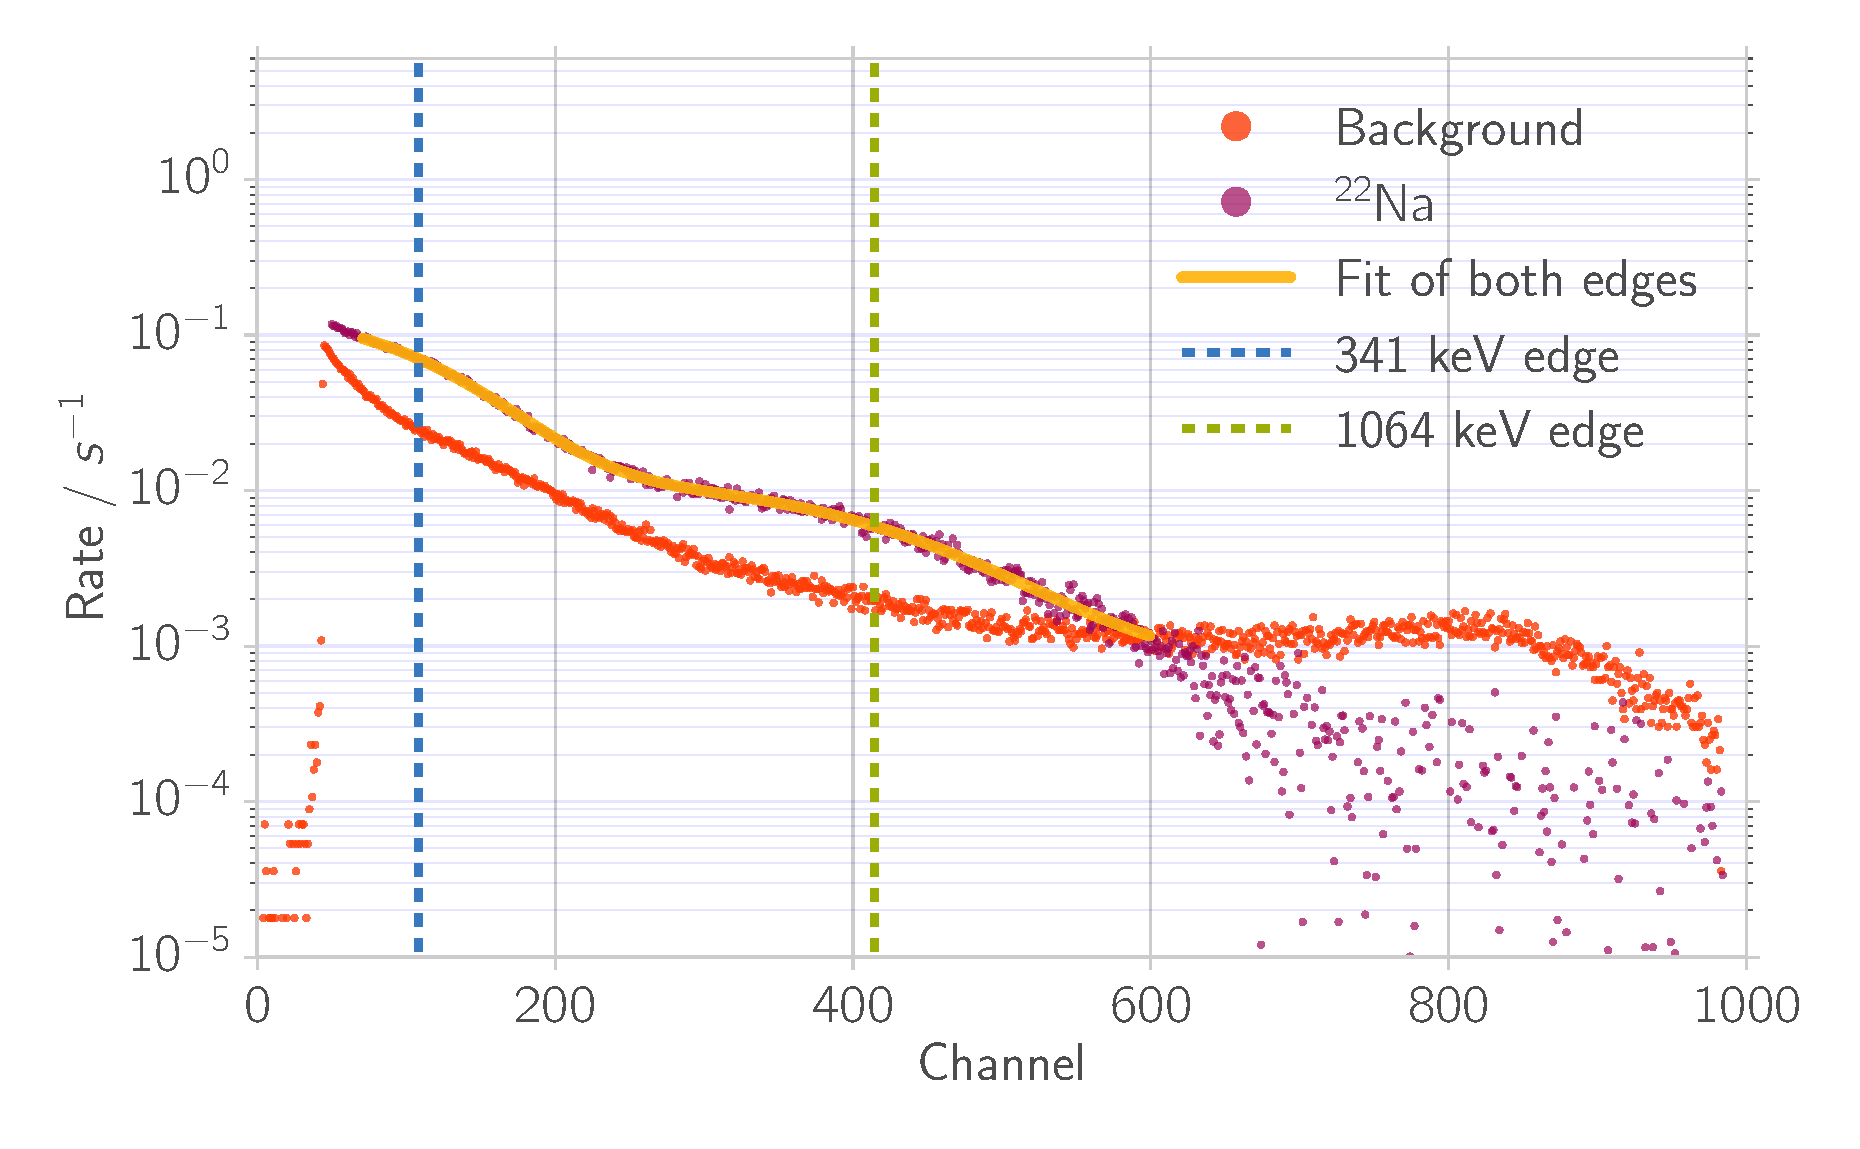
\includegraphics[width=0.9\linewidth]{./analysis/figures/calib_ps_na}
    \caption{Calibration of the PS scintillator with $^{22}$Na sample (measurement time
    16.5 h) with refined background (measurement time 15.6h). As you can notice, rate is 
only fitted for the section in which the background is smaller than the sample. We
subtracted the background rate at each channel for the sample in order not to fit the 
behavior of the noise. The error of the two Compton edges is large (see text) coming
from the fit and their high correlation coefficient.}
\label{fig:calib_ps_na}
\end{figure}
For the $^{137}$ sample we found the Compton at Channel $178.9 \pm 0.3$ 
(notice the much smaller error compared to the $^{22}$Na sample), 
see figure~\ref{fig:calib_ps_cs} for the data and the fit.
\begin{figure}[htpb]
    \centering
    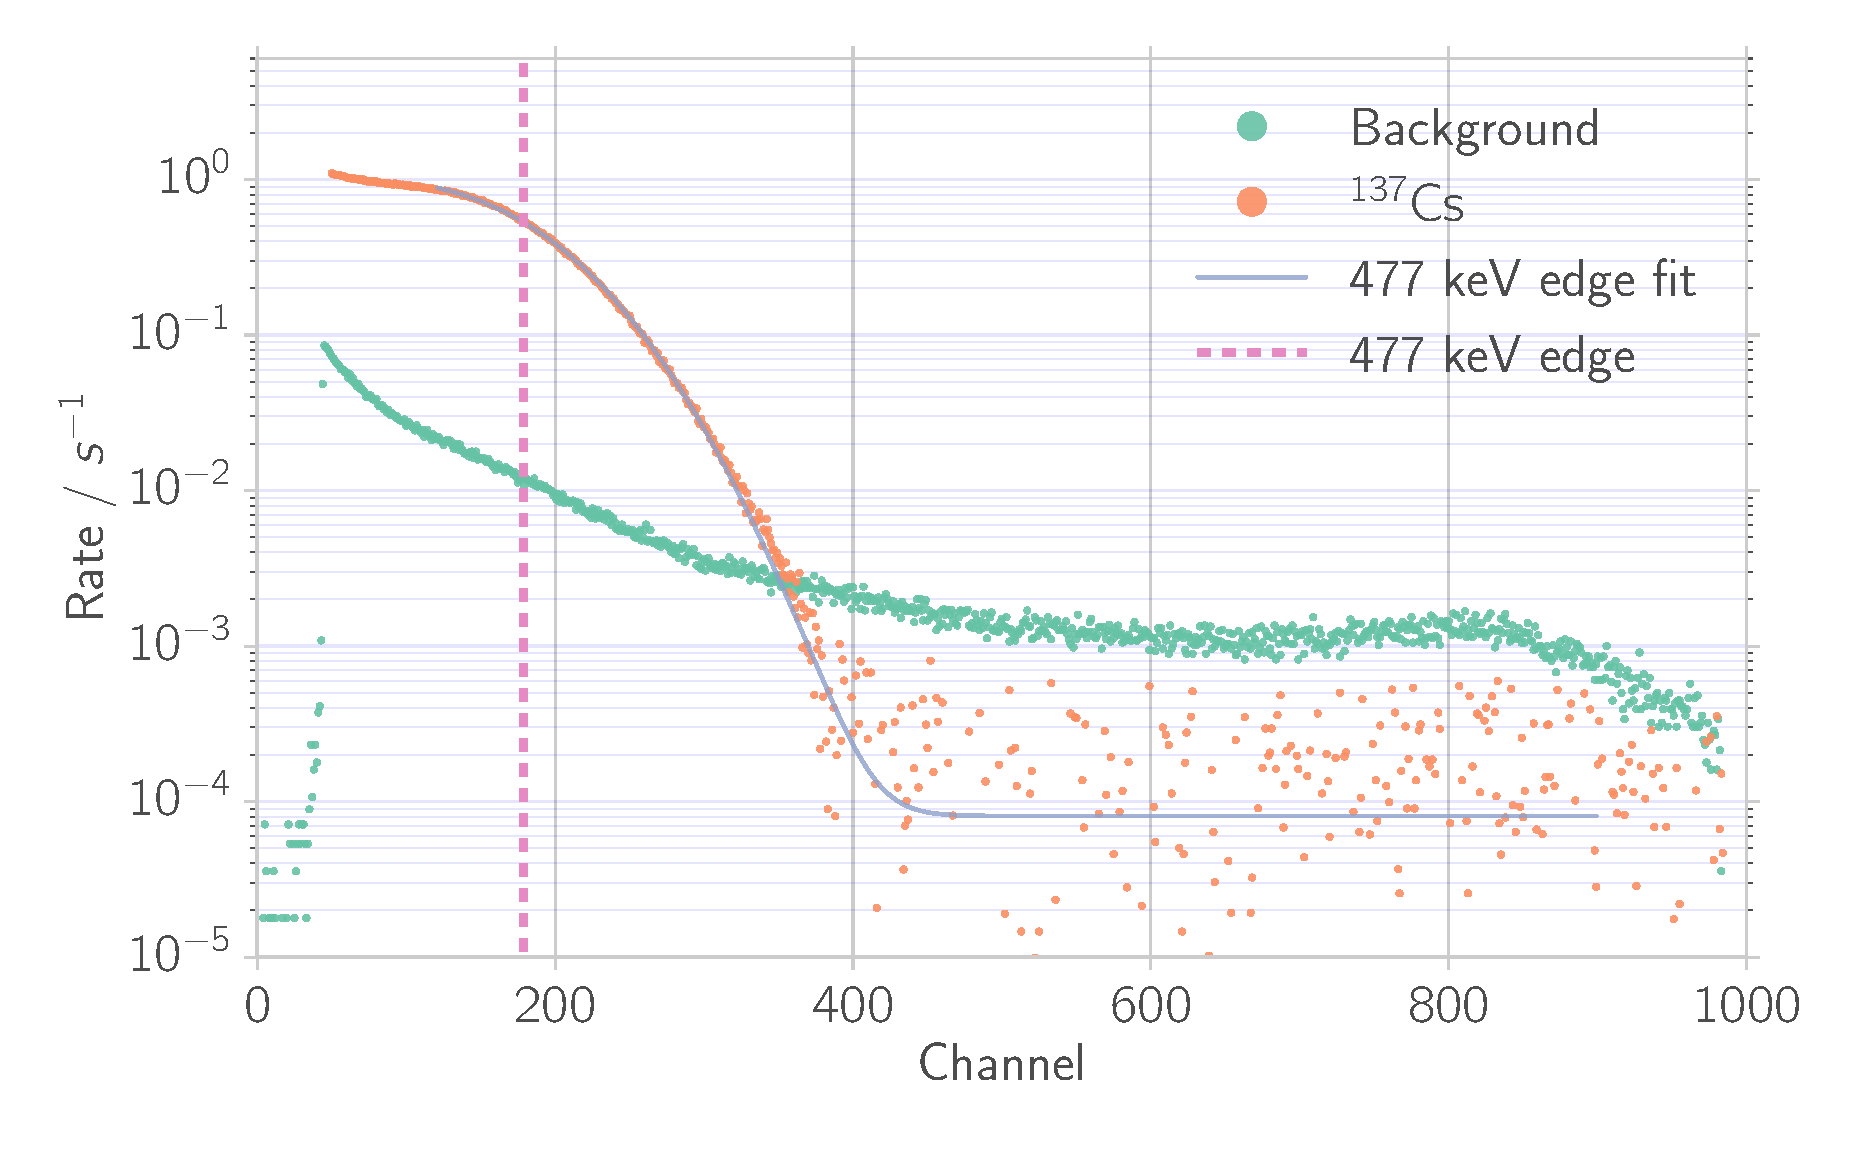
\includegraphics[width=0.9\linewidth]{./analysis/figures/calib_ps_cs}
    \caption{Calibration of the PS scintillator, same as figure~\ref{fig:calib_ps_na}. 
        with $^{137}$Cs sample (measurement time
    6 h) with refined background (measurement time 15.6h, same as before). 
Again we subtracted the background rate at each channel behavior of the noise. }
\label{fig:calib_ps_cs}
\end{figure}

\begin{figure}[htpb]
    \centering
    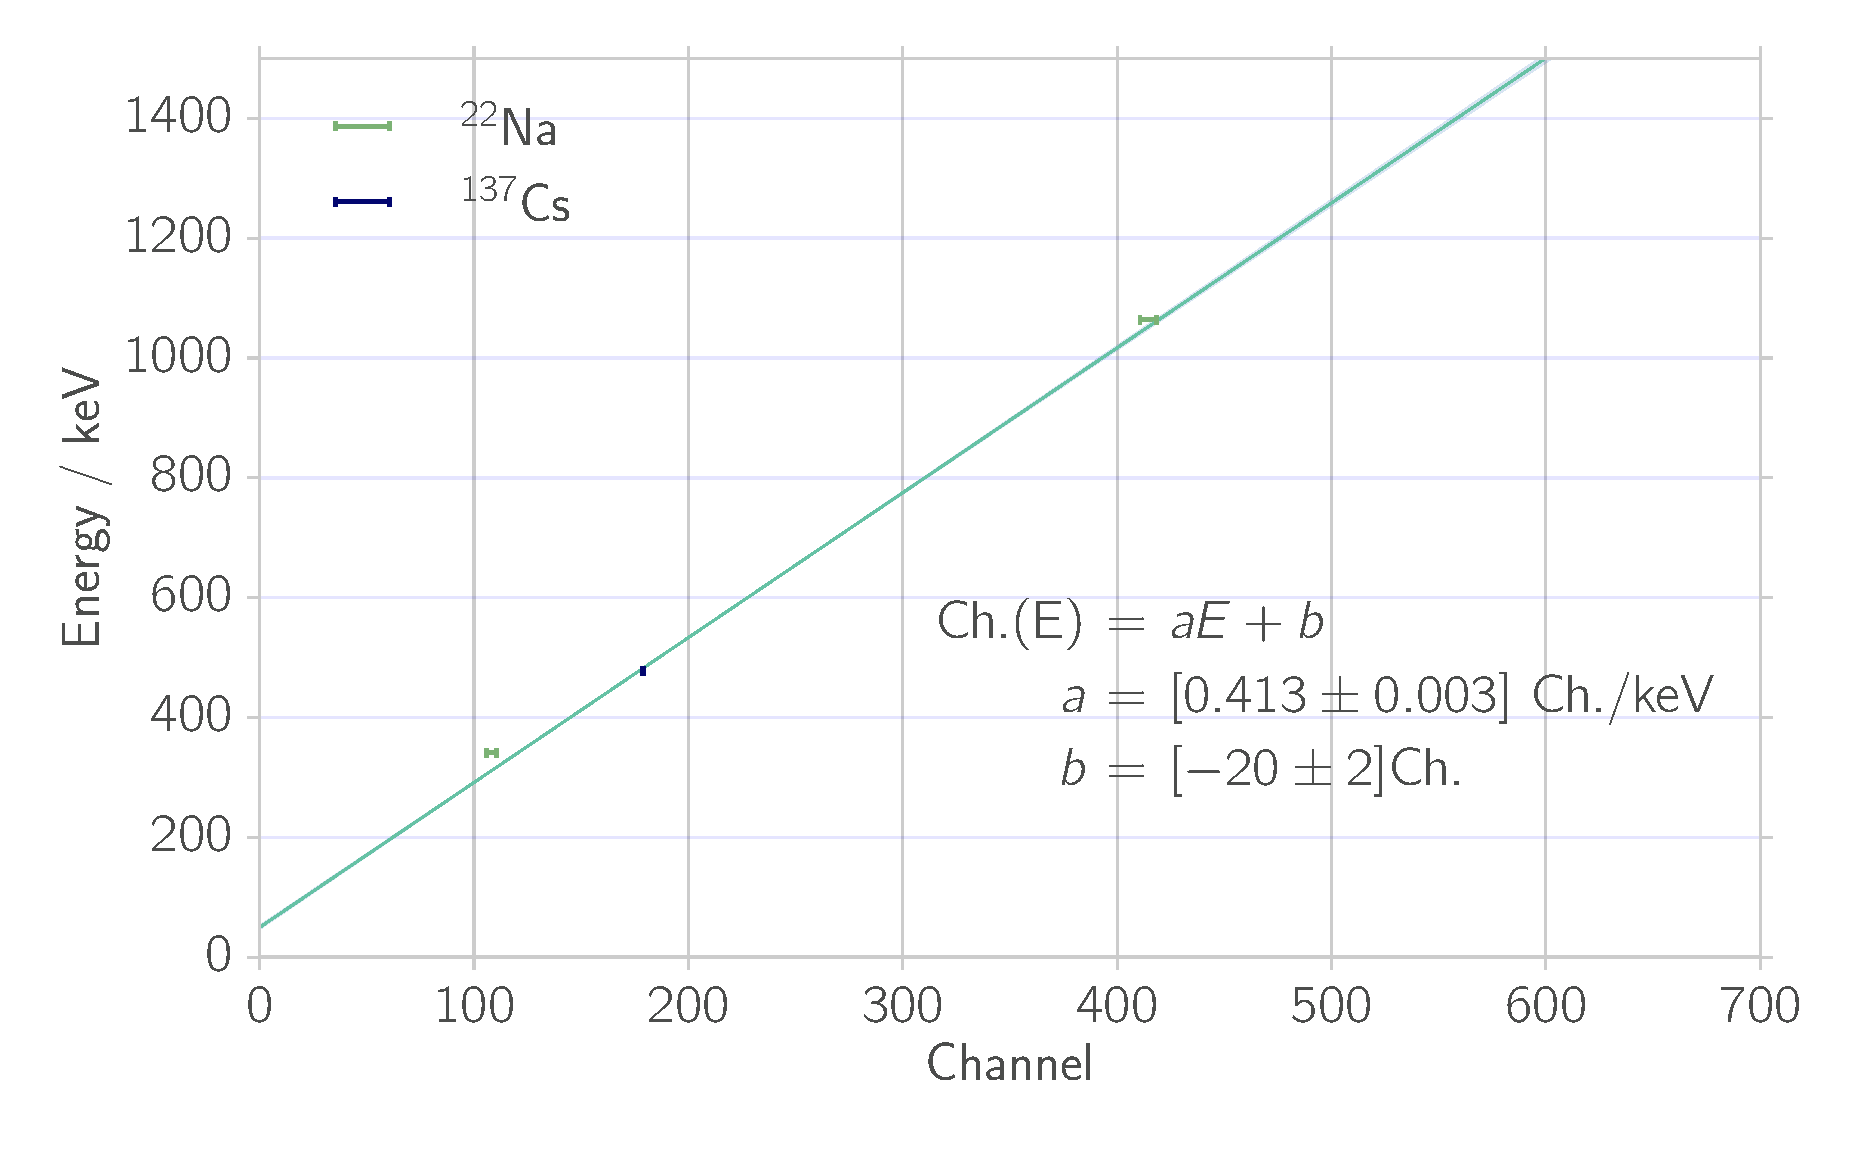
\includegraphics[width=0.9\linewidth]{./analysis/figures/calibration_ps_linear_fit}
    \caption{This is the result of the three Compton edges. We will use this calibration
    for all the following calculations.}
\label{fig:calibration_ps_linear_fit}
\end{figure}
The final result of the linear calibration can be seen in
figure~\ref{fig:calibration_ps_linear_fit}.

\subsection{Calibration of NA scintillator}
\label{sub:calibration_of_na_scintillator}


